\chapter{Introduction}\label{ch:introduction}

\setlength\epigraphwidth{.738\textwidth}
\epigraph{\itshape Life Before Death. Strength Before Weakness. Journey Before Destination.}{Brandon Sanderson, \textit{The Way of Kings.}}

\lettrine{\textcolor{accent_color}{W}}{ho} has never dreamt of a robot friend?
A robot that can help you with your daily tasks, play games with you, help you with your homework or even be your personal assistant?
The idea of having a robotic companion is not new, for it has remained a dream for humanity for a long time.
Since the first mention of the term \textit{robot}~\cite{robot1920}, this aspiration has been only possible in science fiction movies and books.
However, with the recent advancements in robotics and artificial intelligence, we are closer than ever to this reality.
This humble thesis is nothing more than just a small step towards the joint effort of achieving this dream.

Now, how do we create a robot that can be a friend to humans?
This simple question omits a multitude of challenges that need to be addressed.
Some of these challenges include the robot's ability to understand and interact with humans, its ability to learn from its environment, or its ability to adapt to different situations.
However, there is one aspect underlying all these challenges; \textit{movement}:

\begin{itemize}
    \item A robot that understands and interacts with humans \textit{must be able to move} in order to follow the humans and interact with them.
    \item A robot that learns from its environment \textit{must be able to move} in order to explore and gather information.
    \item A robot that adapts to different situations \textit{must be able to move} in order to change its behavior and actions based on the environment.
\end{itemize}

Moreover, it has been thoroughly discussed in the literature that movement is a fundamental aspect of intelligence~\cite{Darwin1871, Arbib2005, Leisman2016, Wolpert2011, Llinas2001}.
This clearly shows that movement is a crucial component of any intelligent system known to us.
If we want to create any intelligent entity that somehow resembles our own intelligence, we must first address the problem of movement.

This thesis is dedicated to the study of movement in robots, specifically in the context of embodied artificial intelligence.
This topic is known as \acrfull{vsn}, in which and agent must navigate in an environment to accomplish certain tasks while only relying on visual information.
On \acrshort{vsn} there is no prior knowledge of the environment or any map that the agent can consult.
The agent must learn to navigate in the environment by exploring it and learning from its own experiences.
It has to understand the scene not only geometrically, but also semantically.
If not, it will not be able to understand the meaning of the objects in the scene and how they relate to each other.
For example, if the agent is placed in a bedroom and asked to find a fridge, it must understand that the fridge is not (typically) in the bedroom and that it must navigate to the kitchen to find it.

\acrshort{vsn} tasks are very challenging, and as one may expect, they typically need a careful design of a complex system that combines multiple components in charge of different aspects of the navigation.
Many works~\cite{newcombe2011, thrun2001, jones2011, sattler2018, Kazerouni2022, campos2021, labbe2022, zhang2018, rosinol2020, jin2023} follow this approach, and they typically rely on a combination of visual perception, semantic understanding, and navigation planning.
However, \acrshort{vsn} can be also formulated as a \acrfull{rl}~\cite{sutton2018} problem.
\acrshort{rl} is a whole artificial intelligent framework that allows an agent to learn how to act in an environment by receiving rewards for its actions.
The rewards are typically defined in terms of the agent's performance in the task, such as reaching a goal or avoiding obstacles.
By following an iterative process within the environment, the agent can learn how to maximize its rewards and complete its tasks.

The main goal of this thesis is to study the \acrshort{rl} and \acrshort{vsn} powerful combination that allows agents to be trained to navigate in an environment.
After intensive training, agents can learn to navigate by trial and error, obtaining rewards that guide them to the goal.
In figure~\ref{fig:abstract_thesis} an abstract representation of the thesis's framework is shown.
In it, an agent, by interacting with the environment, learns to navigate to a goal.
In the environment, even though there is not a map present, the agent can learn to understand the scene and the objects in it.
By these semantic cues, the agent can learn to navigate to the goal, even if it is not visible in the scene.

\begin{figure}
    \centering
    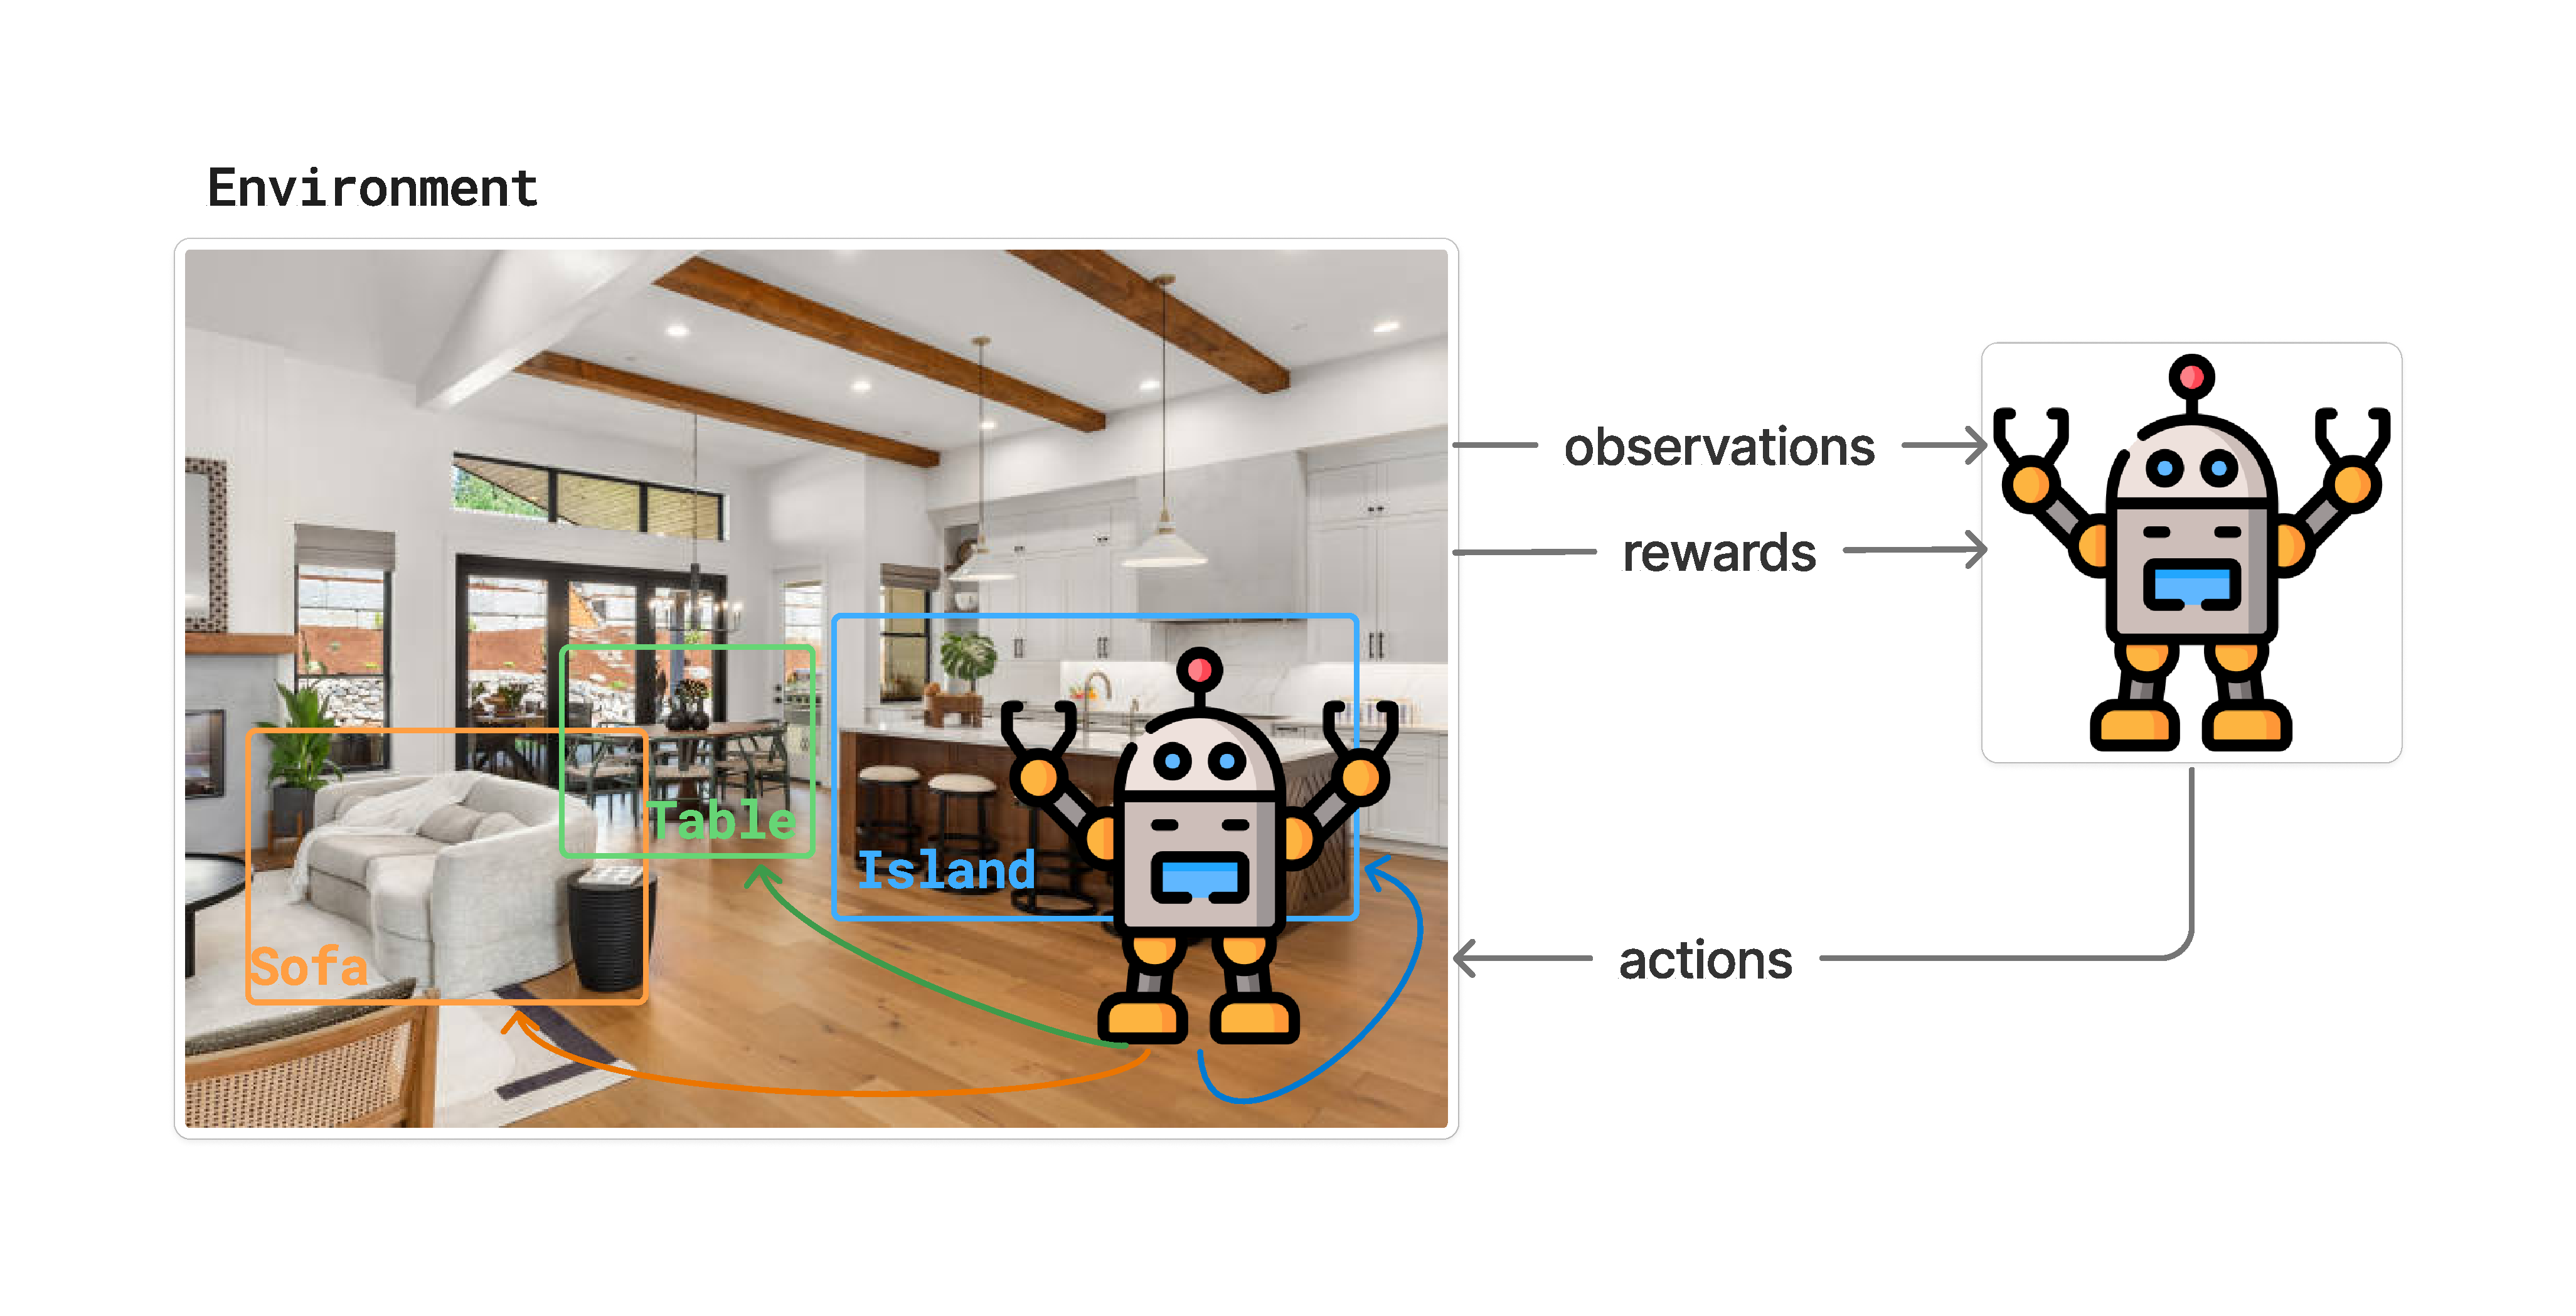
\includegraphics[trim=30 30 30 30, clip, width=\textwidth]{figures/introduction/abstract_thesis}
    \caption{The main goal of this thesis is to study the \acrshort{rl} and \acrshort{vsn} powerful combination that allows agents to be trained to navigate in an environment. After intensive training, agents can learn to navigate by trial and error, obtaining rewards that guide them to the goal.}
    \label{fig:abstract_thesis}
\end{figure}

\section{Motivation}\label{sec:motivation}

This thesis is part of the

\begin{figure}
    \centering
    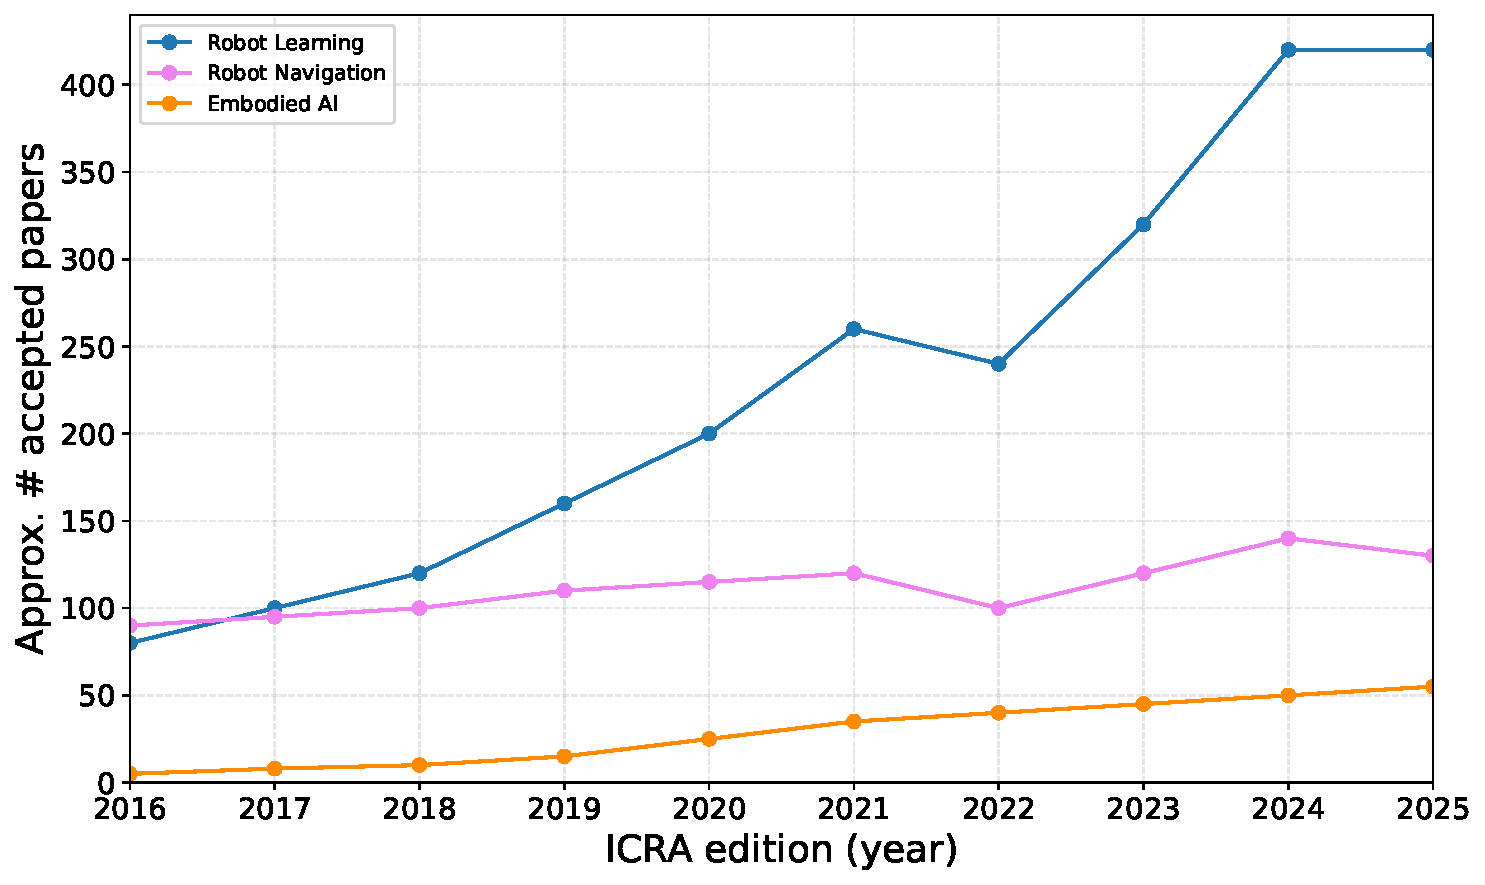
\includegraphics[width=\textwidth]{figures/introduction/icra_papers}
    \caption{A robot friend that can help you with your daily tasks, play games with you, help you with your homework or even be your personal assistant.}
    \label{fig:icra_papers}
\end{figure}


\section{Contributions of the Thesis}\label{sec:contributions-of-the-thesis}


\section{Thesis Structure}\label{sec:thesis-structure}